%!TEX root = main.tex

The results of policy gradient method on CartPole environment is show
in Figure~\ref{fig:pg_cartpole}. Also, a video illustration can be found
in \href{https://gym.openai.com/evaluations/eval_UaXIaMm1QxPGgW45KHtTA#reproducibility}{this link}.
As we can see in both the video and the figure, the game was solved by 
few hundred episodes. This show the effectiveness of policy gradient methods
and we further train a this model in a more complex environment. 

\begin{figure}[h!]
\centering
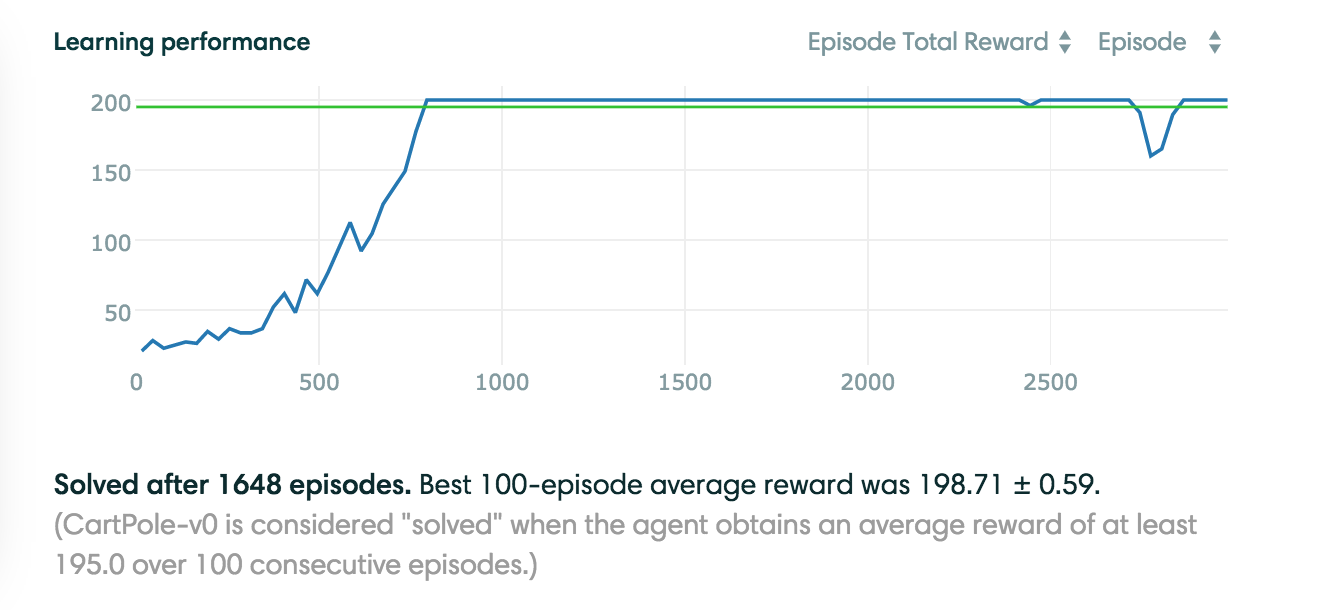
\includegraphics[width=0.49\textwidth]{./fig/pg_cartpole.png} 
\caption{The plot of reward for cartpole game. The x-axis is the number
of episodes it has been trained. The y-axis is the cumulative reward in 
per episode. The higher the better. }
\label{fig:pg_cartpole}
\end{figure}


The performance on Pong game is plot in Figure~\ref{fig:pg_pong} and a video
illustration can be found \href{https://gym.openai.com/evaluations/eval_dODFoXO2S4y5TuUZMX7Nw}{at this link}. As it
shown in the figure, this game requires more than 10000 episodes to get 
a model better than the baseline provided by OpenAI gym. It much more complicated
than the CartPole, since the state and action space is more complex than 
that. The structure of this policy is a single hidden layer with eight
hidden nodes fully connected network and it works. It may perform
better if we use a convolutional network to replace this one, but compared 
the results in dueling DQN, it seems the algorithms of reinforcement learning
itself is more important, other than the specific network architecture. 

\begin{figure}[h!]
\centering
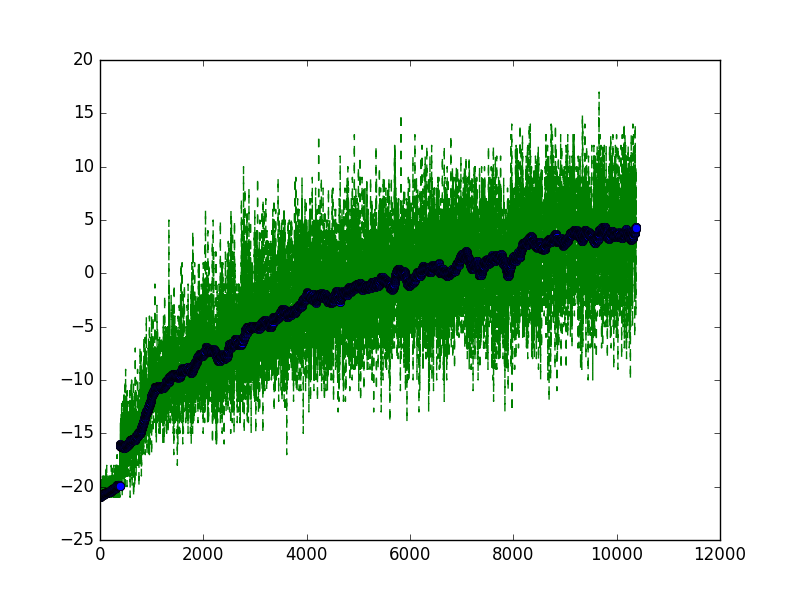
\includegraphics[width=0.49\textwidth]{./fig/pg_pong_rewardsplot.png} 
\caption{The plot of reward for pong game. The x-axis is the number
of episodes it has been trained. The y-axis is the cumulative reward in 
per episode. The higher the better. }
\label{fig:pg_pong}
\end{figure}